\chapter{Project Specification, Planning, and Architecture}

\section{Introduction}
Establishing a robust system requires deep preparation, rigorous specifications, planning, and clean architectural design. This chapter details our functional and non-functional requirements, models the global system needs using a UML Use Case diagram, breaks down the Scrum product backlog, details our development environment, and presents both our infrastructure deployment layout and logical multi-tier application architecture.

\section{Requirements Specification}
To ensure the Predictra Threat Map satisfies academic and operational standards, we captured and defined detailed functional and non-functional requirements.

\subsection{Functional Requirements (RF)}
The platform must support the following nine functional requirements, structured in detail below:

\subsubsection{RF-1: Multi-Feeds Data Ingestion Engine}
\begin{itemize}
    \item \textbf{Description \& Operational Context:} The system must ingest threat events from 9+ external feeds (AlienVault, \allowbreak URLhaus, \allowbreak C2 Tracker, \allowbreak Kaspersky Feodo, \allowbreak Fortinet, \allowbreak Bitdefender, \allowbreak Checkpoint, \allowbreak RansomWatch, \allowbreak and MISP Galaxy), supporting different threat categories (malware, malicious servers, exploits). Collecting data from multiple sources prevents relying on a single vendor, building a more complete threat map. Each external feed utilizes different protocols and data formats. The ingestion layer separates the collection routines, ensuring that a slow query from one feed does not block the collection of others.
    \item \textbf{Use-Case Scenario:} A threat actor registers a new botnet command-and-control server. Within minutes of active staging, the scraper queries the target host, extracts the server details, validates the active listening ports, and pushes the threat indicator into our ingestion pipeline.
    \item \textbf{Inputs:} External threat intelligence feed configurations, API tokens, HTTP endpoints, query rate parameters, connection timeout configurations.
    \item \textbf{Outputs:} Standardized raw threat events JSON packets containing source attributes, raw timestamps, indicator categories, and adversary identification headers.
    \item \textbf{Validation Criteria:} Continuous ingestion from all 9 sources must proceed without data blocking. If an external API goes offline, the scraper must capture the error, log a warning, and schedule a reconnect attempt after a brief delay, preventing server freeze.
\end{itemize}

\subsubsection{RF-2: Geolocation Enrichment Pipeline}
\begin{itemize}
    \item \textbf{Description \& Operational Context:} The backend must automatically find the geographic locations (latitude, longitude, country) of IP addresses using a local geocoding library. Knowing where threats originate helps security teams identify regional attack trends. Because the live stream receives many events per second, resolving locations using online APIs would be too slow and subject to rate limits. Therefore, the geolocation process uses a local database for instant coordinate resolution.
    \item \textbf{Use-Case Scenario:} An incoming exploit log lists the attacker IP \texttt{185.220.101.5}. The geocoder intercepts this address, searches the local IP-to-country database, and resolves the IP to Germany (DE) with coordinates \texttt{51.2993, 9.491}.
    \item \textbf{Inputs:} Raw IP address strings (IPv4 or IPv6 format) extracted from the threat events ingestion queue.
    \item \textbf{Outputs:} ISO two-letter country codes, geocoded Latitude and Longitude decimal coordinates, city name indicators (where available), and Autonomous System Number (ASN) details.
    \item \textbf{Validation Criteria:} Coordinate resolution must execute in low latencies using local caching to avoid external API rate limits. Invalid or private IP blocks (e.g. \texttt{127.0.0.1}) must be mapped to safe default fallback coordinates without raising system exceptions or halting the pipeline execution.
\end{itemize}

\subsubsection{RF-3: Multi-Layer Sector Classification}
\begin{itemize}
    \item \textbf{Description \& Operational Context:} The enrichment engine must dynamically classify threat victims into one of 9 critical business sectors (Healthcare, Finance, Government, Technology, Energy, Education, Telecom, Manufacturing, Retail) using a 5-layer classification engine. This classification allows analysts to filter active threat campaigns targeting their specific vertical. When a cyber threat event occurs, identifying the target industry sector is essential for assessing the systemic risk and cascading impact. For instance, a ransomware attack targeting a financial institution has different regulatory and operational implications compared to a distributed denial-of-service (DDoS) attack targeting a retail website. Since raw feeds rarely contain structured sector tags, the enrichment engine must parse heterogeneous context clues using natural language processing (NLP) keyword matrices, destination port signatures, and historical actor targeting associations to accurately assign a victim sector.
    \item \textbf{Use-Case Scenario:} A RansomWatch scraper indexes an extortion post detailing an attack on "Saint Jude Memorial Hospital." The classifier parses the string, identifies the keyword "Hospital," matches it against the healthcare dictionary, and assigns the target sector to "Healthcare."
    \item \textbf{Inputs:} Attack name, target organization details, destination ports, threat actor profiles, MISP galaxy metadata.
    \item \textbf{Outputs:} Classified target sector name string corresponding to one of the 9 defined critical business sectors.
    \item \textbf{Validation Criteria:} The classification engine must resolve every event within 5 milliseconds. If no sector can be matched via keywords, ports, or metadata, the system must gracefully fall back to the source feed's default sector (such as "Enterprise Technology") to ensure that the event remains categorizable on the threat dashboard.
\end{itemize}

\subsubsection{RF-4: Real-Time Server-Sent Events (SSE) Streaming}
\begin{itemize}
    \item \textbf{Description \& Operational Context:} The server streams geocoded threat events to browsers using a Server-Sent Events (SSE) connection, updating the dashboard instantly without constant polling. Traditional web updates require the browser to request data repeatedly, which is slow and wastes bandwidth. SSE establishes a direct, continuous connection where the server pushes new events to the client. The backend also includes a queue to group and batch incoming threats, ensuring smooth updates.
    \item \textbf{Use-Case Scenario:} A new ransomware victim is indexed. The backend processes the event, enriches it with coordinates, queues it, and immediately flushes it down the open SSE connection, causing the analyst's map to update.
    \item \textbf{Inputs:} Enriched backend threat events from the processing pipeline, active client HTTP connections.
    \item \textbf{Outputs:} HTTP Server-Sent Events (SSE) stream payloads formatted as \texttt{text/}\allowbreak\texttt{event-stream}.
    \item \textbf{Validation Criteria:} Updates must be grouped and flushed at a 300ms interval to protect client browser rendering performance, preventing browser lag from rapid updates. The stream must maintain a keep-alive heartbeat to prevent servers from closing the connection.
\end{itemize}

\subsubsection{RF-5: 3D WebGL Threat Map Visualizer}
\begin{itemize}
    \item \textbf{Description and Context:} The frontend displays an interactive 3D globe showing live attacks as animated curves and pulsating markers, with a toggle to switch to a flat 2D map. A visual threat map is easier to interpret than text logs. The map allows rotation, zooming, and panning. To ensure smooth performance, the visualizer uses hardware acceleration in the browser.
    \item \textbf{Use-Case Scenario:} An analyst mounts the dashboard. A 3D Earth loads in a dark space background, displaying colored lines representing attack vectors between countries.
    \item \textbf{Inputs:} 3D coordinate vectors, attack categories, and time deltas.
    \item \textbf{Outputs:} Interactive 3D visual Earth mesh with glowing arcs, pulsating markers, and country boundary lines.
    \item \textbf{Validation Criteria:} Rendering frame rate must maintain a smooth 60fps under standard attack densities. If the client hardware is low-powered, the system must reduce details to prevent lag.
\end{itemize}

\subsubsection{RF-6: STIX 2.1 Bundle Parser}
\begin{itemize}
    \item \textbf{Description \& Operational Context:} The system must allow analysts to upload standard JSON STIX 2.1 threat intelligence bundles, extract objects (indicators, actors, TTPs), and display them in structured tables. This ensures compliance with global cybersecurity intelligence standards. Standardized threat sharing is essential for collective defense. The Structured Threat Information Expression (STIX) format allows security agencies, CERTs, and private vendors to share threat intelligence without encountering proprietary format blockages. The STIX bundle parser must process complex JSON structures entirely in the browser using client-side JavaScript, ensuring that sensitive enterprise intelligence files are never sent to external servers. The parser must validate the uploaded file structure, extract core STIX domain objects, resolve relationships, and populate the dashboard.
    \item \textbf{Use-Case Scenario:} A government CERT agency releases a STIX bundle concerning a new APT campaign. The analyst uploads the file, extracts the indicators, threat actor profiles, and tools, and reviews them in the structured table.
    \item \textbf{Inputs:} Local STIX 2.1 JSON file uploaded via the dashboard drag-and-drop interface.
    \item \textbf{Outputs:} Isolated maps of STIX objects grouped by threat classes, displayed in interactive, searchable client tables.
    \item \textbf{Validation Criteria:} The parser must validate the JSON schema, ensure the presence of required fields (such as \texttt{spec\_version: "2.1"} and \texttt{type: "bundle"}), and seamlessly support large files (up to 300KB) entirely client-side without locking the browser's main execution thread.
\end{itemize}

\subsubsection{RF-7: MITRE ATT\&CK Kill Chain Mapping}
\begin{itemize}
    \item \textbf{Description \& Operational Context:} The STIX dashboard must map extracted adversary techniques directly into the 12 phases of the MITRE ATT\&CK Cyber Kill Chain, illustrating threat distributions per phase. This categorization assists teams in planning security remediation. The MITRE ATT\&CK matrix is the industry-standard taxonomy for cataloging adversary tactics, techniques, and procedures (TTPs). By mapping ingested STIX attack pattern objects directly to this matrix, the platform provides security teams with immediate visibility into the adversary's operational phase. For example, if a parsed bundle contains an overwhelming number of techniques concentrated in the "Initial Access" phase, defenders know they must focus on perimeter controls. If the techniques are clustered in "Privilege Escalation," internal endpoint security must be audited.
    \item \textbf{Scenario:} The parsed STIX bundle contains techniques like "Spearphishing Link" and "DLL Side-Loading". The matrix groups them under "Initial Access" and "Defense Evasion" respectively, displaying a visual count indicator in the UI grid.
    \item \textbf{Inputs:} Parsed STIX attack pattern objects containing MITRE ATT\&CK \texttt{kill\_}\allowbreak\texttt{chain\_}\allowbreak\texttt{phases} identifiers.
    \item \textbf{Outputs:} Structured 12-phase MITRE ATT\&CK visual matrix showing technique distributions and descriptive popups.
    \item \textbf{Validation Criteria:} Distribution counts per phase must update automatically upon parsing, highlighting the most heavily populated stages to focus mitigation efforts. Malformed or custom phase names must be safely grouped under an "Other / Custom" column to prevent grid rendering failures.
\end{itemize}

\subsubsection{RF-8: Searchable Historical Database Browser}
\begin{itemize}
    \item \textbf{Description \& Operational Context:} The platform must provide a searchable historical log viewer of persisted threat records, filtering by country, target sector, IP address, and free-text regex queries, with paging to protect server performance. Real-time visual monitoring must be backed by a strong historical record system. When a security incident is detected, investigators must query historical logs to perform forensic audits, searching if similar threat vectors have targeted their infrastructure in the past. To ensure high speed, the database queries must leverage indexes on frequently searched fields. The interface must provide paginated views to protect server and client memory from massive document arrays.
    \item \textbf{Use-Case Scenario:} An investigator searches for all "Healthcare" threats originating from "Russia" (RU) during the last week, filtering the results instantly in a searchable table.
    \item \textbf{Inputs:} Search strings, country selection, target sector, pagination index parameters.
    \item \textbf{Outputs:} Paginated BSON threat documents array matching the query filters.
    \item \textbf{Validation Criteria:} Query page size must be bounded (default 50 logs per page) to prevent server memory bloat, with database queries executing in under 50ms using indexing.
\end{itemize}

\subsubsection{RF-9: Target My IP Helper \& Excel Export}
\begin{itemize}
    \item \textbf{Description \& Operational Context:} The history page must integrate a quick-helper to geolocate and query threats targeting the investigator's public IP, alongside a feature to export threat logs into formatted Microsoft Excel files. Analysts often need to run quick sanity checks on their local networks or export forensic evidence for presentation to stakeholders. The "Target My IP" helper queries an external public IP API, geolocates the client, and automatically searches the threat history database to identify if their specific public network IP or neighboring subnet blocks have been logged as active targets by any scraper. The Excel export feature converts current query results into standard XML Spreadsheet formats entirely client-side.
    \item \textbf{Use-Case Scenario:} An analyst wants to see if their current network has been targeted. They click "Target My IP," geolocate themselves, filter the logs, and export the threat list to Excel for a security briefing.
    \item \textbf{Inputs:} Clicked HUD buttons, public IP query results.
    \item \textbf{Outputs:} Geolocated public client IP and formatted Excel spreadsheet downloads.
    \item \textbf{Validation Criteria:} Export must support up to 5,000 logs in a single continuous stream utilizing fast client-side worksheet packages, preventing browser memory exhaustion.
\end{itemize}

\subsection{Non-Functional Requirements (RNF)}
To satisfy system reliability, performance, and aesthetic standards, five non-functional requirements were established:

\begin{subsubsection}{RNF-1: High Frame-Rate and UI Fluidity}
The 3D globe should run smoothly at 60 frames per second (FPS). The frontend must implement adaptive checks, dynamically reducing visual details if the frame rate drops, ensuring that map controls remain responsive.
\end{subsubsection}

\begin{subsubsection}{RNF-2: Minimal Memory Footprint}
The client dashboard must manage memory efficiently. The system uses a circular buffer with a maximum capacity of 10,000 events to store data. This buffer overrides old events in-place, keeping memory usage constant and avoiding performance stutters.
\end{subsubsection}

\begin{subsubsection}{RNF-3: Self-Cleaning Storage \& Time-To-Live (TTL)}
The database growth must be bounded. Old threat records must automatically expire and prune from the database after a 30-day Time-To-Live (TTL) interval, avoiding billing overages on free cloud database tiers.
\end{subsubsection}

\begin{subsubsection}{RNF-4: Database Storage Quota Guard}
The backend monitors the database collection size. If database storage exceeds 500 MB, the server automatically stops database writes and switches to in-memory streaming to prevent database errors.
\end{subsubsection}

\begin{subsubsection}{RNF-5: Glassmorphism UI Theme}
The interface implements a modern dark theme design, utilizing semi-transparent panel styles and colors based on threat severity, which reduces eye strain and provides a clean visual workspace.
\end{subsubsection}

\section{System Needs Modeling}
To define the system boundary, we identified the primary actors and modeled their interactions with the global platform using a UML Use Case diagram.

\subsection{Identification of Actors}
We identified two main actors interacting with our system:
\begin{itemize}
    \item \textbf{External Threat Feeds (System Actor):} Ingests raw cyber threat logs via HTTP REST APIs, SSE feeds, or WebSockets. It acts as the primary data supplier.
    \item \textbf{Security Analyst (Human Actor):} Interacts with the frontend dashboard to monitor geolocated threat vectors, explore history, export data, and upload/explore STIX 2.1 threat intelligence bundles.
\end{itemize}

\subsection{Global Use Case Diagram}
The global interactions are illustrated in the UML Use Case diagram in Figure~\ref{fig:global_usecase}.

\begin{figure}[H]
\centering
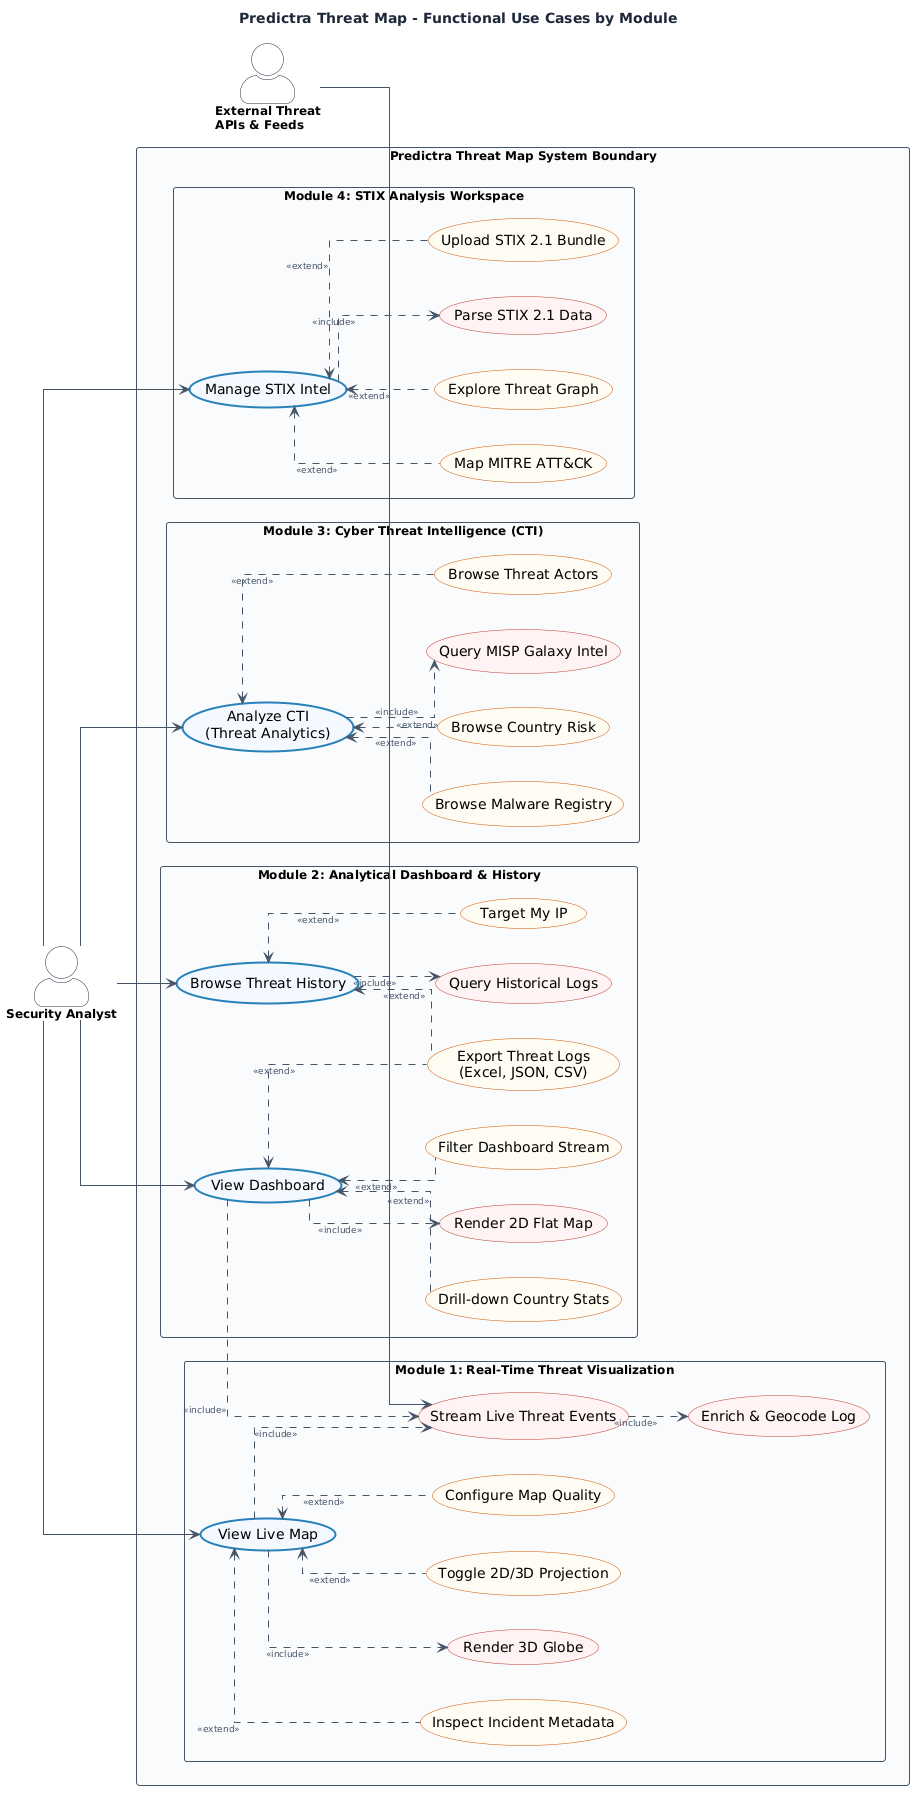
\includegraphics[width=\textwidth,height=0.85\textheight,keepaspectratio]{assets/global_usecase.png}
\caption{UML Global Use Case diagram for the Predictra CTI platform.}
\label{fig:global_usecase}
\end{figure}

The specific functional workflows of these use cases are summarized in Table~\ref{tab:global_uc_desc}.

\begin{table}[H]
\centering
\small
\arrayrulecolor{charcoal!30}
\rowcolors{2}{cyberblue!5}{white}
\begin{tabularx}{\textwidth}{>{\raggedright\arraybackslash}p{3.2cm}>{\raggedright\arraybackslash}p{3.5cm}X}
\hline
\rowcolor{charcoal}
\thc{Base Use Case} & \thc{Included / Extending} & \thc{Main Workflow \& Interaction Details} \\
\hline
View Live Map &
\textbf{Includes:} Stream Live Events, Render 3D Globe \newline
\textbf{Extends:} Toggle 2D/3D Projection, Configure Map, Inspect Metadata &
Security Analyst mounts the map view. The frontend initiates the WebGL globe render loop and hooks into the Server-Sent Events (SSE) client stream. Optional controls allow altering atmospheric/trail quality, flattening coordinates to 2D Mercator, and hovering over bezier arcs to see raw metadata. \\
\midrule
View Dashboard &
\textbf{Includes:} Stream Live Events, Render 2D Flat Map \newline
\textbf{Extends:} Filter Dashboard, Drill-down Country, Export Logs &
Security Analyst opens the flat command center view. System displays grid panels containing real-time metrics, sparklines, and maps. Analyst can query events using regex, click countries to see drill-down reports, or export the active buffer to JSON, CSV, or formatted Excel sheets. \\
\midrule
Browse Threat History &
\textbf{Includes:} Query Historical Logs \newline
\textbf{Extends:} Target My IP, Export Logs &
Security Analyst searches the persistent database. System queries MongoDB Atlas collections. Helper features allow automated public IP geolocation checks (Target My IP) to query matching subnet logs and client-side formatting for Excel spreadsheet exports. \\
\midrule
Analyze CTI \newline (Threat Analytics) &
\textbf{Includes:} Query MISP Galaxy \newline
\textbf{Extends:} Browse Actors, Browse Malware, Browse Country Risk &
Security Analyst accesses the threat intelligence portal. The system retrieves stored MISP Galaxy templates. The analyst filters APT groups by country attribution or target sector, audits ransomware encryption details, and views geographical vulnerability heatmaps. \\
\midrule
Manage STIX Intel &
\textbf{Includes:} Parse STIX 2.1 \newline
\textbf{Extends:} Upload STIX, Map MITRE &
Security Analyst mounts the STIX 2.1 analysis environment. The analyst uploads a JSON bundle, parsed client-side. The frontend maps adversary patterns into the 12 phases of the MITRE ATT\&CK Cyber Kill Chain. \\
\hline
\end{tabularx}
\caption{Detailed descriptions of the global primary use cases and their relationships.}
\label{tab:global_uc_desc}
\end{table}

\clearpage

\section{Project Management with Scrum}
As described in Chapter 1, we implemented the Agile Scrum methodology to pilot the design and realization.

\subsection{Product Backlog}
The features requested by the Product Owner were broken down into four distinct sprint backlogs:
\begin{itemize}
    \item \textbf{Sprint 1 (Ingestion Backend):} Setup Express backend server, database schemas, MongoDB Atlas connections, 9 parallel REST/stream scrapers, and the 5-layer sector classification pipeline. Focus on high-throughput database inserts and robust API connection pooling.
    \item \textbf{Sprint 2 (Visualizer Frontend 3D Earth):} Develop the Express SSE feed endpoint with 300ms queue, establish the Zustand store on the React frontend, and build the 3D procedural WebGL Earth Canvas with bloom rendering, bezier fly-arcs, and pulsating markers. Target a smooth 60fps orbital rotation.
    \item \textbf{Sprint 3 (STIX Analysis Workspace):} Create the frontend STIX 2.1 JSON parser and implement the MITRE ATT\&CK Kill Chain mapping. Focus on client-side parsing performance and kill chain validation.
    \item \textbf{Sprint 4 (Analytics, History \& Performance Polish):} Setup the historical log browser, code "Target My IP" geolocator, integrate MISP threat actor datasets, write Excel export streams, and implement performance safeguards (RingBuffer, Zustand throttler, and adaptive FPS sampling drops).
\end{itemize}

\subsection{Previsional Gantt Chart}
Our chronological sprint schedule is modeled in Figure~\ref{fig:gantt_chart} using a timeline chart.

\begin{figure}[H]
\centering
\begin{tikzpicture}[x=0.95cm, y=0.85cm]

  % ─── constants ────────────────────────────────────────────────────
  \def\nrows{4}   % number of sprint rows
  \def\ncols{12}  % total weeks
  \def\lw{2.6}    % left-label column width (in x-units, shifted)

  % ─── alternating row backgrounds ──────────────────────────────────
  \fill[gray!8]  (0, 0) rectangle (\ncols, 1);
  \fill[white]   (0, 1) rectangle (\ncols, 2);
  \fill[gray!8]  (0, 2) rectangle (\ncols, 3);
  \fill[white]   (0, 3) rectangle (\ncols, 4);

  % ─── outer border ─────────────────────────────────────────────────
  \draw[charcoal!40, line width=0.7pt] (0,0) rectangle (\ncols, 4);

  % ─── vertical week separator lines ────────────────────────────────
  \foreach \w in {1,2,...,11} {
    \draw[gray!30, line width=0.35pt] (\w, 0) -- (\w, 4);
  }

  % ─── horizontal row separator lines ───────────────────────────────
  \foreach \r in {1,2,3} {
    \draw[gray!30, line width=0.35pt] (0, \r) -- (\ncols, \r);
  }

  % ─── header row ───────────────────────────────────────────────────
  \fill[charcoal!12] (0,4) rectangle (\ncols, 4.55);
  \draw[charcoal!40, line width=0.7pt] (0,4) rectangle (\ncols, 4.55);
  \foreach \w in {1,...,12} {
    \node[font=\footnotesize\bfseries, text=charcoal]
      at (\w-0.5, 4.275) {W\w};
  }

  % ─── row label column header ───────────────────────────────────────
  % (drawn to the left of x=0)
  \fill[charcoal!12] (-\lw, 0) rectangle (0, 4.55);
  \draw[charcoal!40, line width=0.7pt] (-\lw, 0) rectangle (0, 4.55);
  \draw[charcoal!40, line width=0.5pt] (-\lw, 4) -- (0, 4);
  \node[font=\footnotesize\bfseries, text=charcoal] at (-\lw/2, 4.275) {Sprint};

  % row dividers in label column
  \foreach \r in {1,2,3} {
    \draw[gray!30, line width=0.35pt] (-\lw, \r) -- (0, \r);
  }

  % ─── sprint row labels ─────────────────────────────────────────────
  \node[font=\small\bfseries, text=charcoal, align=center]
    at (-\lw/2, 3.5) {\#1};
  \node[font=\small\bfseries, text=charcoal, align=center]
    at (-\lw/2, 2.5) {\#2};
  \node[font=\small\bfseries, text=charcoal, align=center]
    at (-\lw/2, 1.5) {\#3};
  \node[font=\small\bfseries, text=charcoal, align=center]
    at (-\lw/2, 0.5) {\#4};

  % ─── Sprint bars ──────────────────────────────────────────────────
  % Sprint 1: Weeks 1-3, Row 4 (y=3..4)
  \fill[cyberblue!30, rounded corners=3pt]
    (0.08, 3.14) rectangle (2.92, 3.86);
  \draw[cyberblue!70, line width=0.8pt, rounded corners=3pt]
    (0.08, 3.14) rectangle (2.92, 3.86);
  \node[font=\scriptsize\bfseries, text=charcoal, align=center,
         text width=2.6cm]
    at (1.5, 3.5) {Harvester\\Backend};

  % Sprint 2: Weeks 4-6, Row 3 (y=2..3)
  \fill[cyberblue!48, rounded corners=3pt]
    (3.08, 2.14) rectangle (5.92, 2.86);
  \draw[cyberblue!80, line width=0.8pt, rounded corners=3pt]
    (3.08, 2.14) rectangle (5.92, 2.86);
  \node[font=\scriptsize\bfseries, text=charcoal, align=center,
         text width=2.6cm]
    at (4.5, 2.5) {3D Visualizer};

  % Sprint 3: Weeks 7-9, Row 2 (y=1..2)
  \fill[cyberblue!66, rounded corners=3pt]
    (6.08, 1.14) rectangle (8.92, 1.86);
  \draw[cyberblue!90, line width=0.8pt, rounded corners=3pt]
    (6.08, 1.14) rectangle (8.92, 1.86);
  \node[font=\scriptsize\bfseries, text=charcoal, align=center,
         text width=2.6cm]
    at (7.5, 1.5) {STIX Parser};

  % Sprint 4: Weeks 10-12, Row 1 (y=0..1)
  \fill[cyberblue!88, rounded corners=3pt]
    (9.08, 0.14) rectangle (11.92, 0.86);
  \draw[cyberblue, line width=0.8pt, rounded corners=3pt]
    (9.08, 0.14) rectangle (11.92, 0.86);
  \node[font=\scriptsize\bfseries, text=white, align=center,
         text width=2.6cm]
    at (10.5, 0.5) {Analytics\\\& Polish};

\end{tikzpicture}
\caption{Previsional Gantt Chart of development sprints.}
\label{fig:gantt_chart}
\end{figure}

\section{Work Environment}
To support development and testing, we established a standardized hardware and software environment.

\subsection{Hardware Environment}
\begin{itemize}
    \item \textbf{Development Workstation:} Intel Core i7 12th Generation Processor, 16 GB DDR4 RAM, 512 GB NVMe SSD, Nvidia GeForce RTX 3060 Laptop GPU (essential for rendering and debugging high-velocity WebGL atmospheric fragment shaders and real-time bloom post-processing filters without interface lagging).
    \item \textbf{Staging Test Server:} Dual-core Virtual Private Server representing cloud staging infrastructure.
\end{itemize}

\subsection{Software Environment and Development Tools}
\begin{itemize}
    \item \textbf{Operating System:} Windows 11 Home for developer environments, Linux Ubuntu Server 22.04 LTS for cloud API staging processes.
    \item \textbf{IDE:} Visual Studio Code (VS Code) with TypeScript ESLint, Git, and LaTeX Workshop extensions.
    \item \textbf{Database Inspection:} MongoDB Compass for inspecting Mongoose models and TTL indexes, and Robo 3T.
    \item \textbf{API Testing:} Postman for constructing mock threat streams and auditing Server-Sent Events headers.
\end{itemize}

\subsection{Stack and Frameworks Comparative Analysis}
The selection of our development stack was not arbitrary; it was the result of a rigorous architectural evaluation designed to balance the competing demands of high-throughput backend data harvesting and ultra-smooth, lightweight frontend WebGL rendering. Every framework and language was scrutinized against standard industry alternatives to ensure optimal resource efficiency.

\subsubsection{Core Languages: Type Safety vs. Volatile Scripting}
For backend development, we used JavaScript to handle the incoming data formats which can vary in structure. On the client side, we implemented TypeScript to provide structure and type-checking, preventing runtime errors that could crash the interface.

\subsubsection{Backend Environment: Node.js/Express vs. Java Spring Boot / Go}
We selected Node.js with Express instead of heavy enterprise environments like Java Spring Boot or Go:
\begin{itemize}
    \item \textbf{Comparison with Spring Boot:} Spring Boot allocates substantial server resources for each connection. In our case, where we maintain continuous connections for streaming threat data, this would consume significant memory.
    \item \textbf{Comparison with Go:} While Go is fast, Node.js provides a large ecosystem of libraries for database mapping, geocoding, and REST requests, allowing faster development.
    \item \textbf{Node.js Advantages:} Node.js is designed to handle thousands of concurrent client connections efficiently under a low memory footprint, making it ideal for streaming threat feeds in real-time.
\end{itemize}

\subsubsection{Frontend Engine: React 19 \& Vite 7 vs. Webpack / Next.js}
For the client-side interface, we used React with Vite instead of Webpack or Next.js:
\begin{itemize}
    \item \textbf{Next.js:} Next.js is optimized for page pre-rendering and SEO, which is not needed for a real-time visual application where all data updates dynamically in the browser.
    \item \textbf{Vite vs. Webpack:} Webpack compiles all assets before starting, which is slow. Vite compiles code on-demand, providing faster startup times and quicker updates during development.
\end{itemize}

\subsubsection{3D Graphics: Three.js and React Three Fiber (R3F)}
To display the 3D globe with many overlapping lines and markers, we used Three.js via React Three Fiber (R3F). R3F allows building 3D meshes using React components, handling resizing and camera controls automatically while keeping the performance high.

\subsubsection{State Management: Zustand 5 vs. Redux Toolkit}
To manage real-time threat data in the browser, we chose Zustand over Redux Toolkit. Redux triggers full-page render updates, which slows down performance when receiving multiple events per second. Zustand allows direct updates to the 3D canvas components, keeping the interface smooth.

\subsubsection{Data Persistence: MongoDB Atlas BSON vs. SQL Relational Databases}
For database storage, we utilized MongoDB instead of relational databases like PostgreSQL or MySQL. Relational databases require rigid table structures, which is difficult because threat data from different scrapers contains different fields. MongoDB allows storing flexible document structures, making it easier to integrate new feeds.

\subsubsection{Technology Stack Comparative Summary Matrix}
To formalize the architectural rationale behind our technology choices, a detailed comparison matrix evaluating our selected stack against traditional enterprise alternatives is presented in Table~\ref{tab:tech_stack_comparison}.

\begin{table}[H]
\centering
\small
\arrayrulecolor{charcoal!30}
\rowcolors{2}{cyberblue!5}{white}
\begin{tabularx}{\textwidth}{>{\raggedright\arraybackslash}p{2.2cm}>{\raggedright\arraybackslash}p{2.5cm}>{\raggedright\arraybackslash}p{2.5cm}X}
\hline
\rowcolor{charcoal}
\thc{Layer / Component} & \thc{Selected Technology} & \thc{Traditional Alternative} & \thc{Architectural Rationale for Selection} \\
\hline
\textbf{Runtime Engine} & Node.js LTS (v20) \& Express 5 & Java Spring Boot & Asynchronous non-blocking event-driven loop vs heavy Thread-per-Request. Scalable for open SSE streams under low memory. \\
\textbf{State Management} & Zustand 5 & Redux Toolkit & Slice-based reactive updates outside React DOM rendering vs full-tree dispatches. Essential for preserving 60fps WebGL rendering. \\
\textbf{Graphics Engine} & Three.js \& React Three Fiber & Vanilla HTML5 Canvas & Declarative component composition, GPU acceleration, SLERP math, and custom GLSL vertex/fragment shaders. \\
\textbf{Client Build Tool} & React 19 \& Vite 7 & Angular \& Webpack & Native ESM during dev, instant startup, fast HMR updates vs slow dependency pre-compilation graphs. \\
\textbf{Data Persistence} & MongoDB Atlas (BSON) & PostgreSQL / MySQL & Dynamic schemaless BSON documents for heterogeneous CTI logs vs rigid relational tables requiring heavy migrations. \\
\hline
\end{tabularx}
\caption{Comprehensive architectural comparison of selected vs alternative technologies.}
\label{tab:tech_stack_comparison}
\end{table}

\section{Architectural Design}
To guarantee maximum horizontal scalability and system responsiveness under high threat ingestions, we adopted a clean, modular multi-tier architecture.

\subsection{Deployment Architecture}
The system deployment model is structured into three cloud layers:
\begin{enumerate}
    \item \textbf{Frontend Layer (Vercel CDN):} The single-page application is hosted on Vercel's global Content Delivery Network. The configuration file `vercel.json` intercepts client requests and handles API proxy rewrites directly, as summarized in Table~\ref{tab:vercel_proxy} (with the full production configuration file detailed in Appendix D.1).
    \item \textbf{Backend Layer (Virtual Cloud VM):} The Node.js Express server runs as a continuous service managed by PM2 on a secure virtual instance. PM2 clusters the Node process across multiple virtual CPU cores, routing client requests and handling automated crash recoveries.
    \item \textbf{Database Layer (MongoDB Atlas Cluster):} persistence is offloaded to a replicated MongoDB Atlas cloud cluster, handling scalable BSON document writes.
\end{enumerate}

\begin{table}[H]
\centering
\small
\arrayrulecolor{charcoal!30}
\rowcolors{2}{cyberblue!5}{white}
\begin{tabular}{ll}
\hline
\rowcolor{charcoal}
\thc{Source Match Rule} & \thc{Target VM Service Endpoint} \\
\hline
\texttt{/api/:path*} & \texttt{http://api:3001/api/:path*} \\
\hline
\end{tabular}
\caption{Frontend Reverse-Proxy Routing Configuration.}
\label{tab:vercel_proxy}
\end{table}

\subsection{System Package Component Architecture}
To ensure clean separation of concerns, our physical system is organized into decoupled modules, as illustrated in the UML Component diagram in Figure~\ref{fig:component_diagram}.

\begin{figure}[H]
\centering
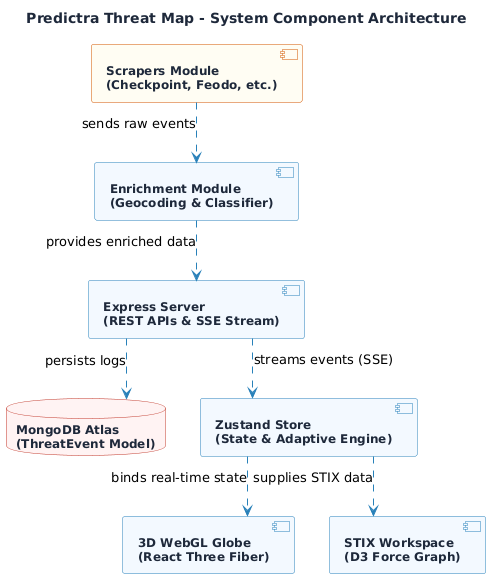
\includegraphics[width=0.95\textwidth]{assets/component_diagram.png}
\caption{UML Component diagram of the Predictra CTI system.}
\label{fig:component_diagram}
\end{figure}

\subsection{Application Logical Architecture}
The Predictra Threat Map's internal logic is partitioned into 4 distinct tiers, as illustrated in the logical architecture diagram in Figure~\ref{fig:logical_architecture}.

\begin{figure}[H]
\centering
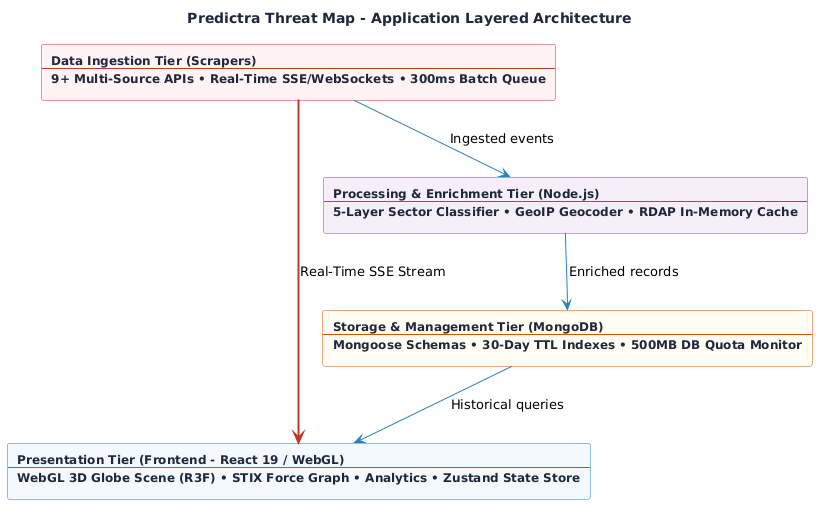
\includegraphics[width=0.95\textwidth]{assets/multi_tier_architecture.png}
\caption{Predictra platform multi-tier layered application architecture.}
\label{fig:logical_architecture}
\end{figure}

This multi-tier structure enforces strict data-flow boundaries:
\begin{itemize}
    \item \textbf{Data Isolation:} Ingestion processes are decoupled from main database queries. Scrapers fetch raw feeds independently, queuing items to prevent memory locks.
    \item \textbf{Decoupled Presentation:} The WebGL client consumes the live stream directly via the SSE pipeline. This bypasses long-term storage routes, ensuring that high database writes do not interfere with 3D canvas responsiveness.
\end{itemize}

\subsection{Global Class Diagram}
To model the static structure of the Predictra CTI system, we designed a Global Class Diagram that illustrates the key logical modules, their core attributes, operational methods, and structural relationships. The diagram is illustrated in Figure~\ref{fig:global_class_diagram}.

\begin{figure}[H]
\centering
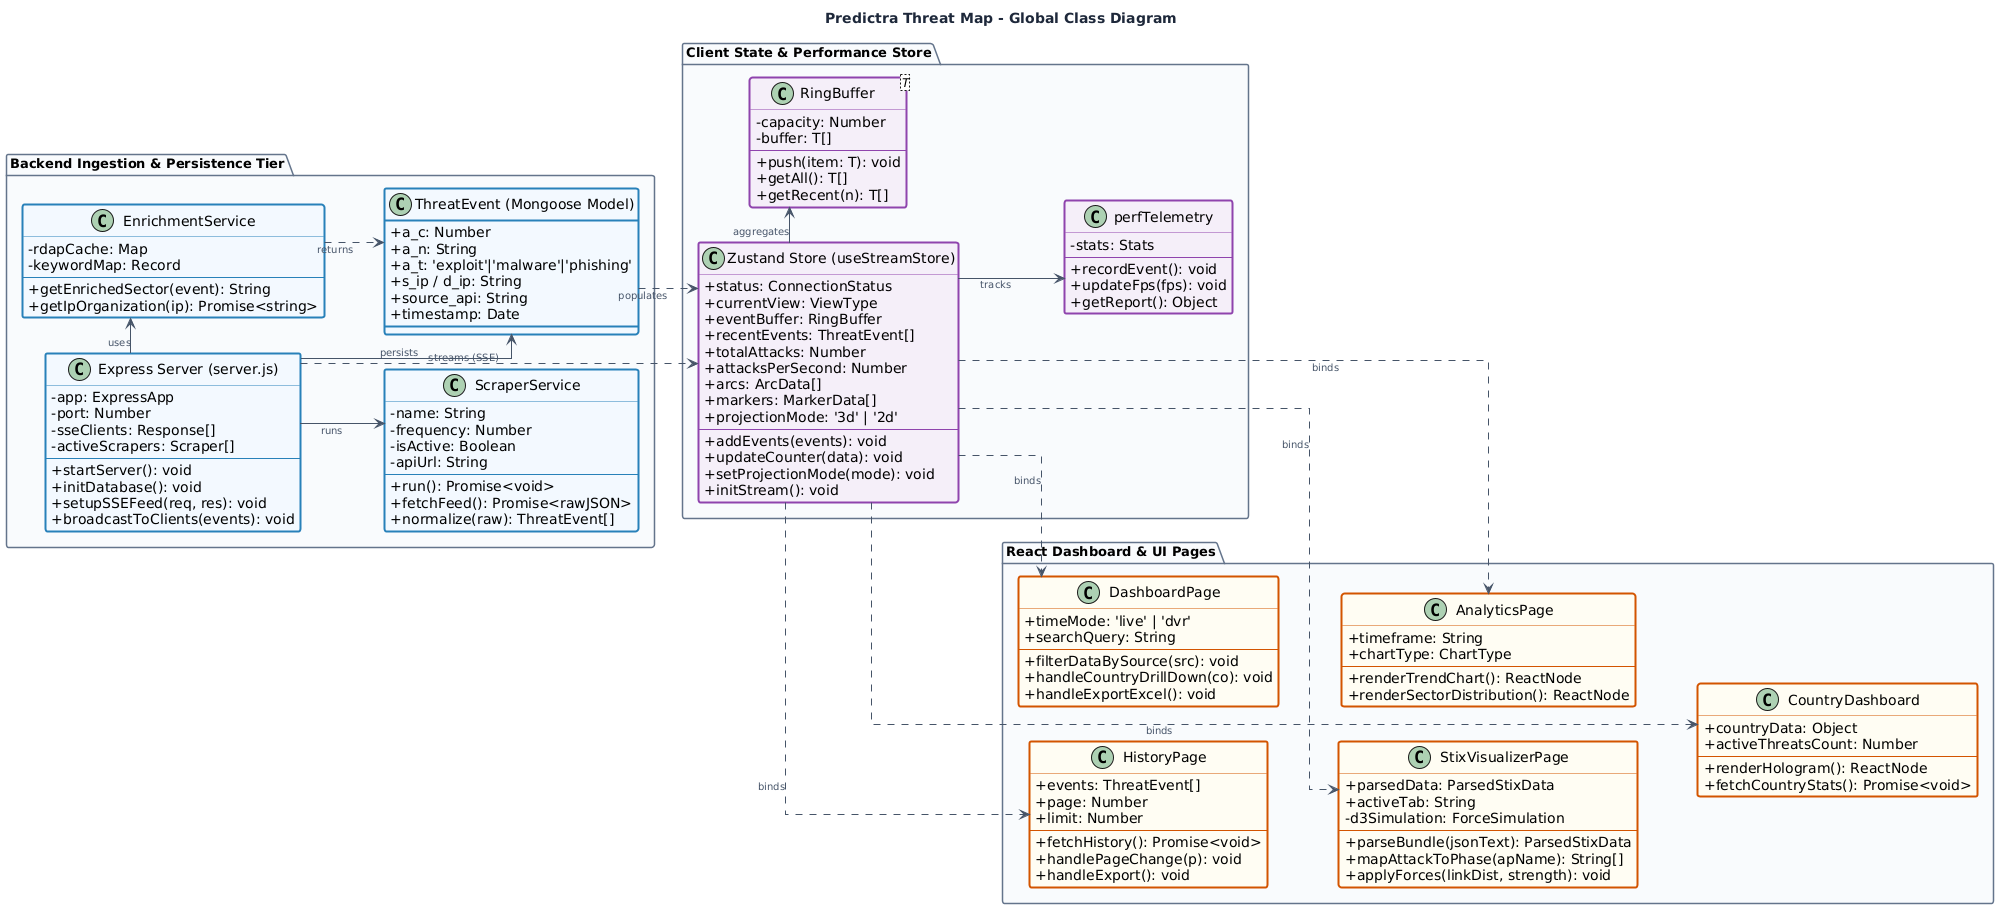
\includegraphics[width=0.95\textwidth]{assets/global_class_diagram.png}
\caption{UML Global Class diagram of the Predictra CTI system.}
\label{fig:global_class_diagram}
\end{figure}

The structural design modeled in Figure~\ref{fig:global_class_diagram} highlights several key object-oriented associations, compositions, and structural dependencies across the three main tiers of our application:
\begin{itemize}
    \item \textbf{Backend Ingestion \& Persistence Tier:} The central \texttt{Express Server} instantiates and schedules multiple concurrent \texttt{ScraperService} instances (e.g. \texttt{Urlhaus}, \texttt{AlienVault}, \texttt{MispGalaxy}, \texttt{Ransomwatch}). As threat telemetry is gathered, it is processed via the \texttt{EnrichmentService} which resolves network organizations and classifies critical infrastructure sectors. The server then persists the resulting dataset using the Mongoose \texttt{ThreatEvent} data model, maintaining standard index rules.
    \item \texttt{Zustand Store} and performance utilities: The client-side \texttt{useStreamStore} acts as a real-time reactive state manager. To handle incoming threat stream data without memory leaks or high garbage collection cycles, the store encapsulates a circular \texttt{RingBuffer} class structure and tracks performance through the custom instrumented \texttt{perfTelemetry} class.
    \item \textbf{React Views Tier:} React pages and tab elements represent the core view controllers. The \texttt{DashboardPage}, \texttt{HistoryPage}, \texttt{AnalyticsPage}, \texttt{StixDashboard}, and \texttt{CountryDashboard} subscribe to the Zustand store state slices and bind to specific endpoints (like \texttt{/api/history} and \texttt{/api/stats}) to drive layout changes and charts.
\end{itemize}

\section{Conclusion}
This chapter established the complete blueprints of our CTI platform. Having documented the functional/non-functional specifications, structured the Scrum timelines, cataloged our dev environment, and detailed our layered deployment and application logical architectures, we proceed to Chapter 3 to document the deep implementation details and UML structures of our first Release.
